\chapter{Simulation Overview}
\paragraph*{}
For our simulation, this is just a recap for our simulation. We have three Turtlebots in the Webots simulation with a square arena. Now each robot faces parallel to the x-axis, which results in the theta starting orientation of 0. This will act as a calibration step of our odometry to ensure that every robot has a theta of 0. Now, after the simulation starts, the robot will move around randomly, given a polynomial. In fact, it will scratch the random part. It will actually just follow a polynomial, which usually in this case just turns slightly left. The simulation is set up in a way that the two robots will see the yellow object, which if one of the robots sees the yellow object, it will stop. And sends a signal to the two robots, which is simultaneously sharing the location data. So, all the three robots are aware of each other's location, giving a mesh communication system. So, even if the two robots detect the yellow object at the same time, it will go through a queue to reduce the issue of the race condition. After the first robot sees the object, it will sense the coordinates. Because it already knows the location of the two other robots, it will calculate the path for them to go to the robot and grasp it. So, therefore, the main one, or the host, or the robot that found the object, will calculate the path for the two other robots, send it to the robot, and the two other robots will send a message that says that it understands and received the message. And the three robots will follow the set path and go to the end destination. Of course, for the path following, it has a PID, which takes the error of the distance to each waypoint. That is used to drive the velocity of the motors or how much force it is giving out. And when the object reaches the cylinder, or the object detected, it will stop. The main challenges of the simulation was the three robots communicating to each other, of getting the data correct.

\begin{figure}
    \centering
    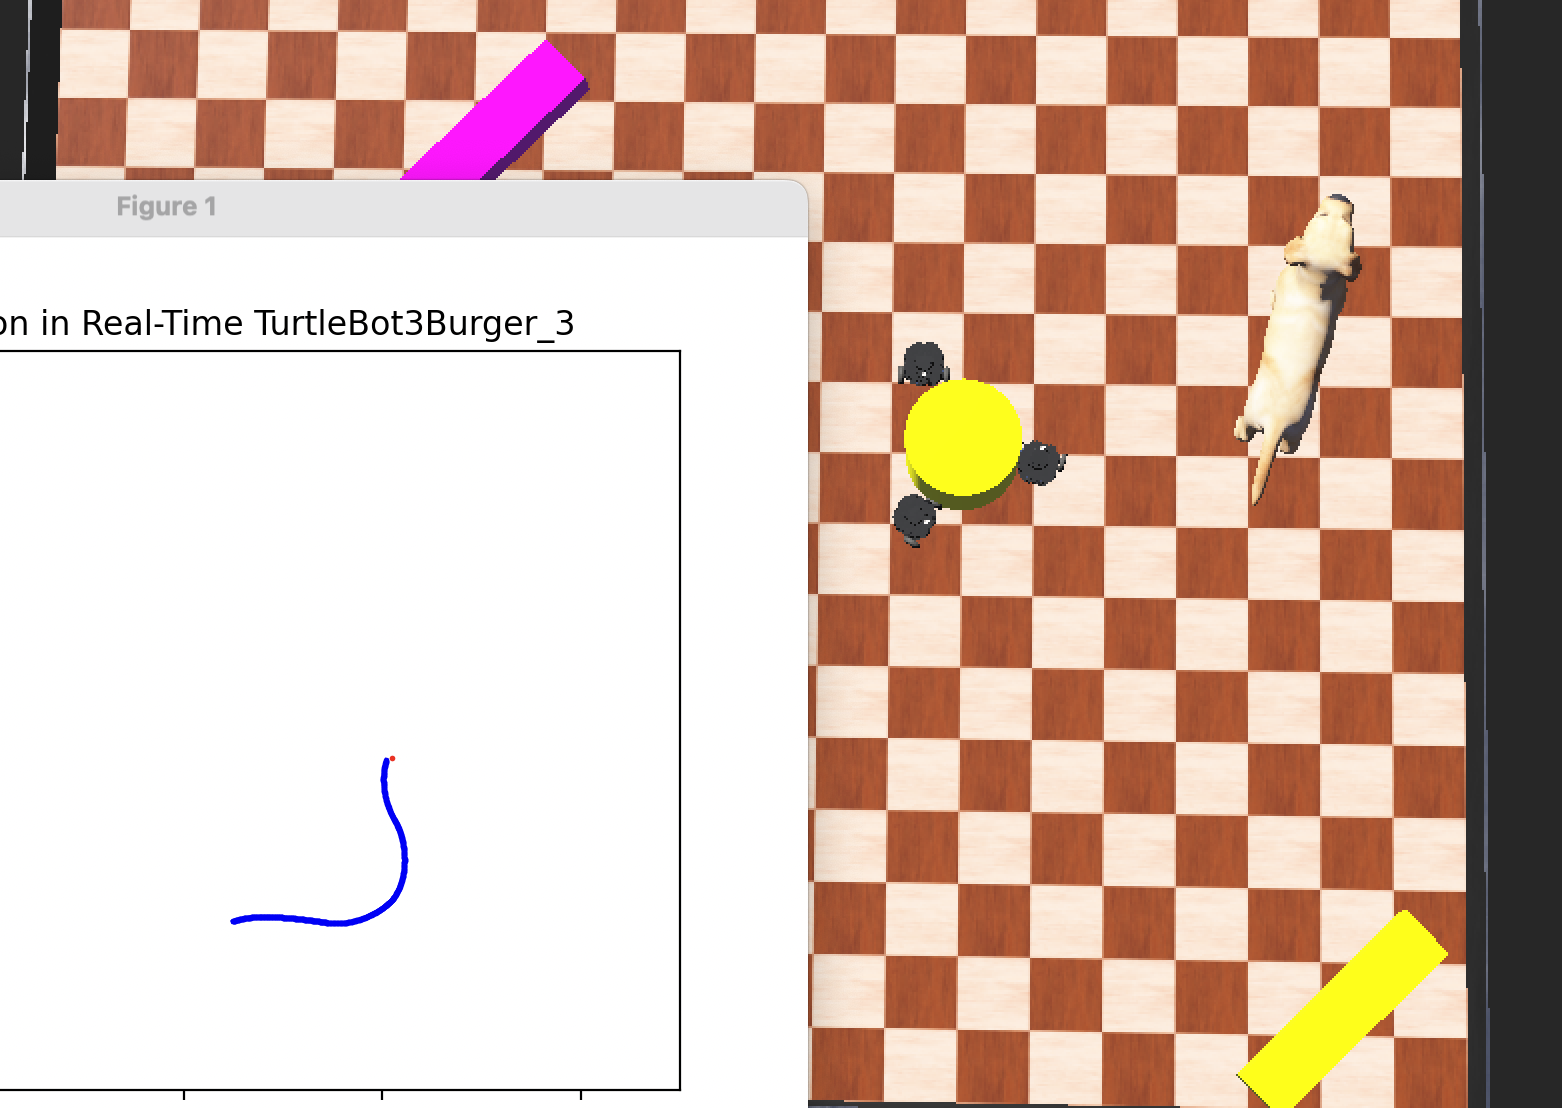
\includegraphics[width=0.5\linewidth]{assets/images/simulation_overview/sim_1.png}
    \caption{Path of the TurtleBotBurger3 after receiving path to follow from the main controller.}
    \label{fig:object detection figure 1} 
\end{figure}

\begin{figure}
    \centering
    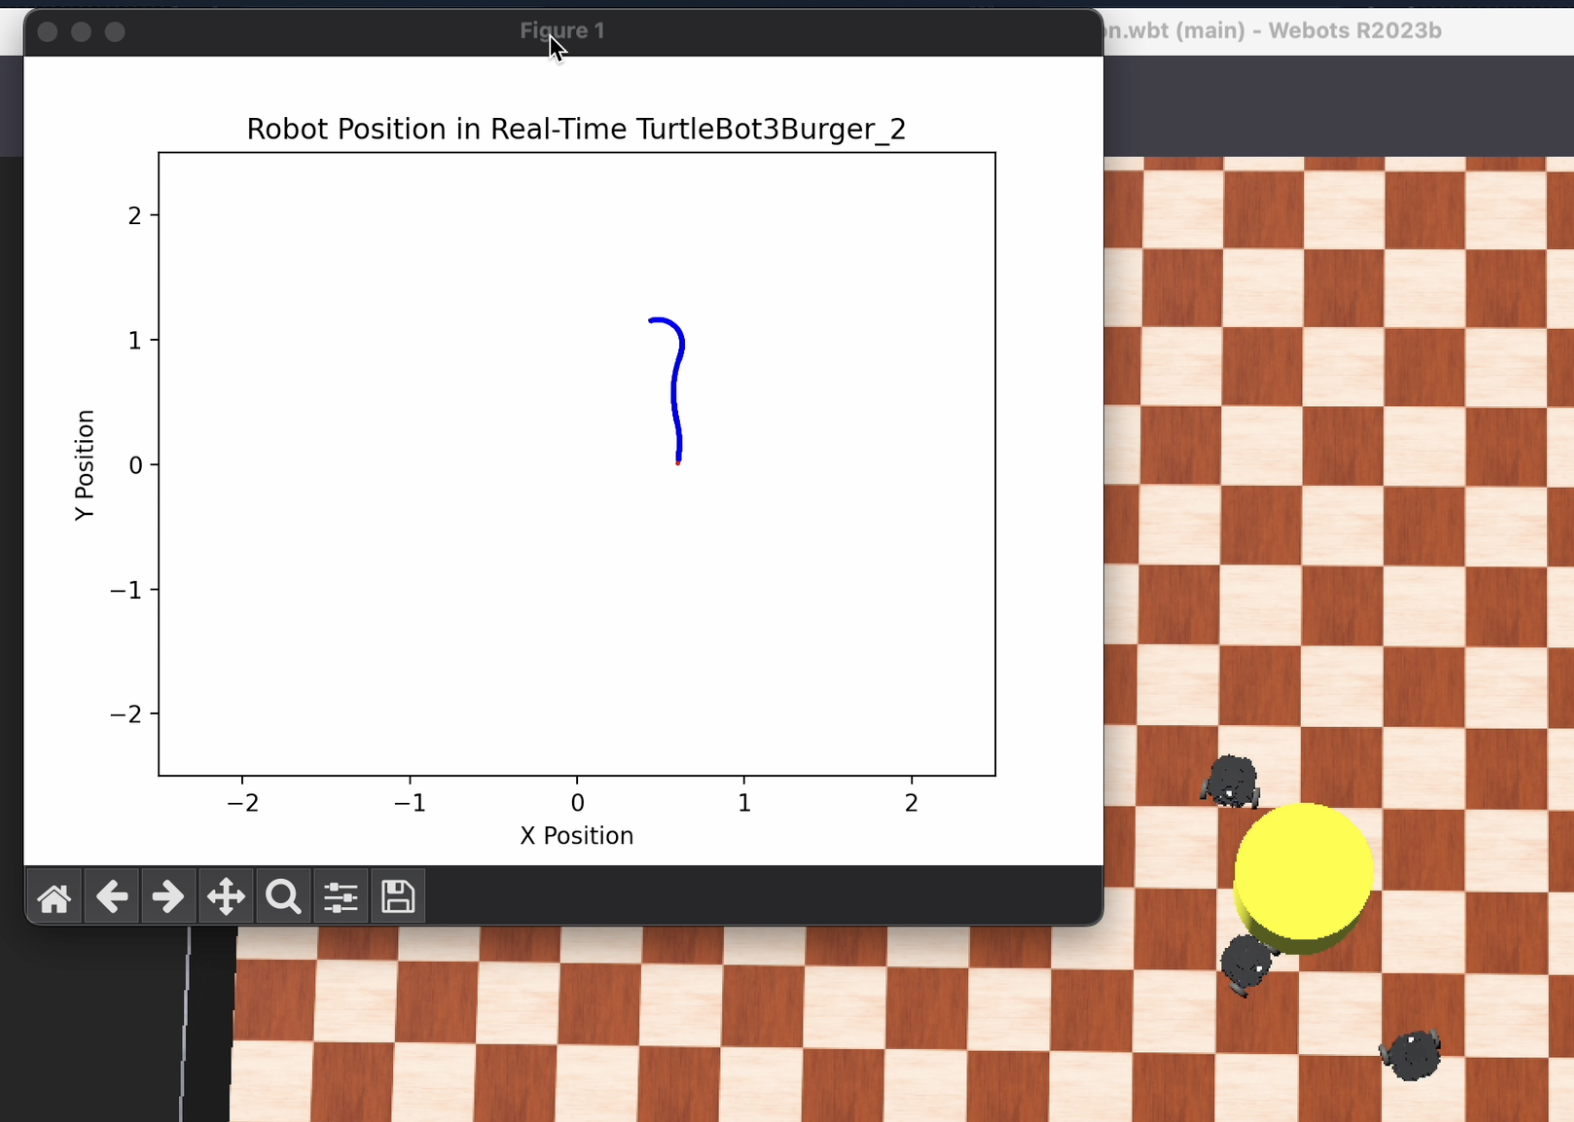
\includegraphics[width=0.5\linewidth]{assets/images/simulation_overview/sim_2.png}
    \caption{3 robots converging to the pre-determined position.}
    \label{fig:object detection figure 2}
\end{figure}

\begin{figure}
    \centering
    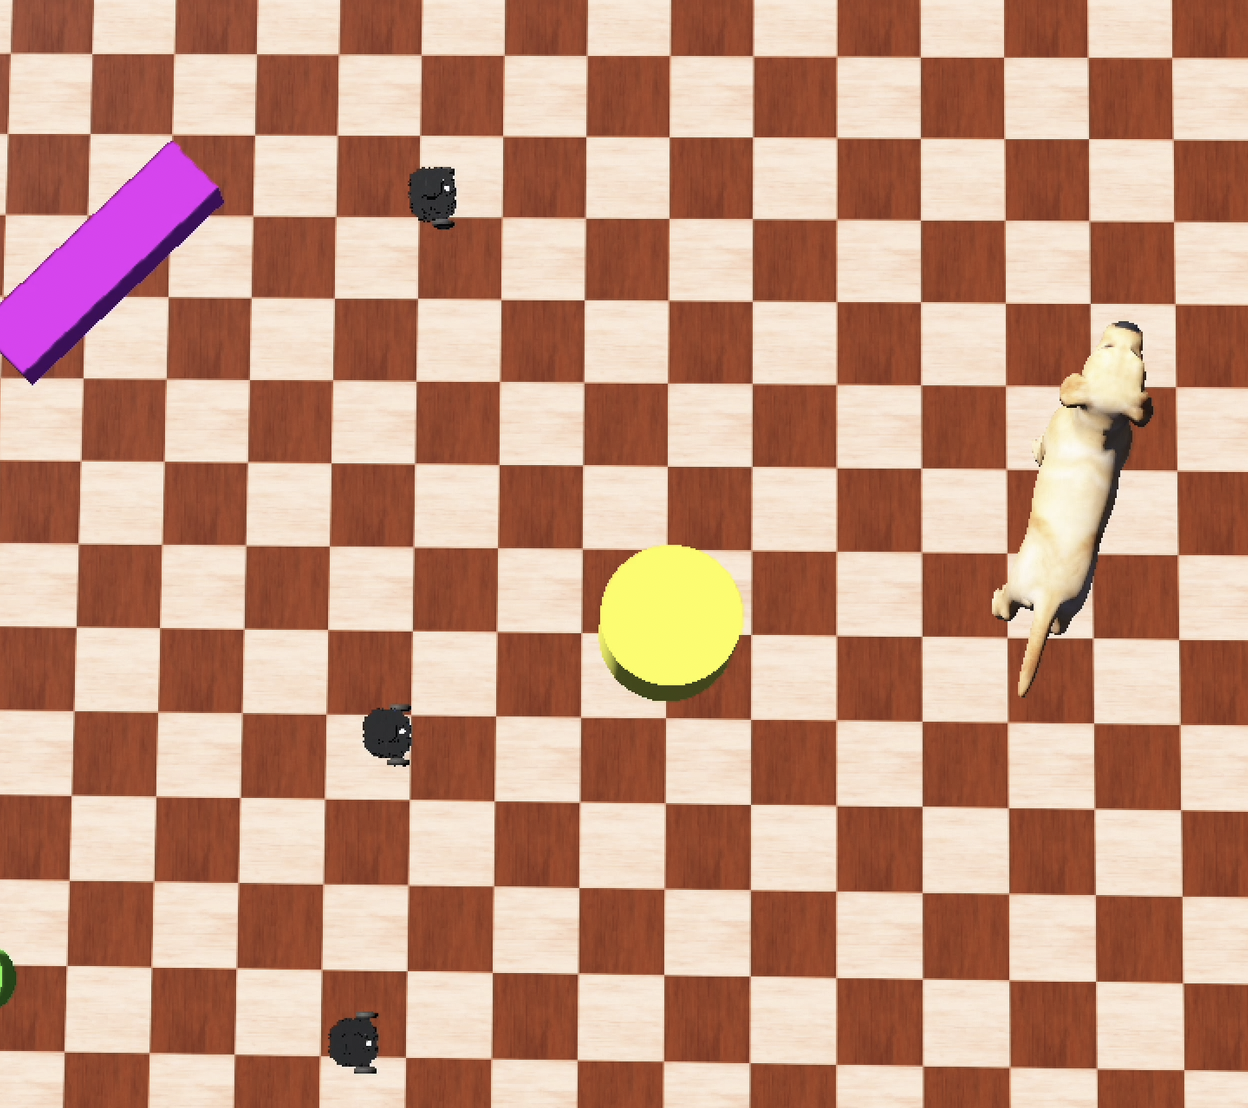
\includegraphics[width=0.5\linewidth]{assets/images/simulation_overview/sim_3.png}
    \caption{3 robot simply moving until an yellow object is found}
    \label{fig:object detection figure 2}
\end{figure}